\documentclass[main.tex]{subfiles}

\title{Lær Python dag 1 - modul 2}
\subtitle{Conditionals, funktioner}

\begin{document}

\maketitle

\begin{frame}{Indhold}
  \setbeamertemplate{section in toc}[sections numbered]
  \tableofcontents[hideallsubsections]
\end{frame}


%\section{Recap}
%\begin{frame}[fragile]{Hvad har I lært sidste modul?}
%	\begin{itemize}
%		\item Hvad er python?
%		\item Hvad er typer?
%		\item Hvad er variabler?
%		\item Hvad er kommentarer?
%		\item Hvad har I ellers lært?
%	\end{itemize}
%\end{frame}

\section{Conditionals}
%%%% TODO: fix < og >
\begin{frame}[fragile]{Boolske udtryk - sandt og falsk}
	Vi har ofte brug for at sammenligne ting, for at tage beslutninger. For at sammenligne om ting er lig med hinanden bruges dobbelt lig med, ==. 

\begin{columns}
	\column{0.4\textwidth}
	\begin{lstlisting}[style=python]
print(4 == 4)
print(4 == 2)
print(type(True))
	\end{lstlisting}
\pause
	\column{0.4\textwidth}
	\begin{lstlisting}[style=python]
True
False
<type 'bool'>
	\end{lstlisting}

\end{columns}

\end{frame}

\begin{frame}[fragile]{Boolske udtryk - sandt og falsk}
Her er en liste af sammenligningsoperatorer.
\begin{lstlisting}[style=python]
x == y   # er x lig med y?
x != y   # er x forskellig fra y?
x < y    # er x mindre end y?
x <= y   # er x mindre end eller lig med y?
x > y
x >= y
\end{lstlisting}

Eksempler, alle giver True.
\begin{lstlisting}[style=python]
4 > 2
2+2 == 4
3 != 4
"hej" == "h" + "ej"
\end{lstlisting}
\end{frame}

\begin{frame}[fragile]{Boolske udtryk - sandt og falsk}
	Man kan også bruge \texttt{not} til at skifte \texttt{True} til \texttt{False} og omvendt:
	\begin{columns}
		\column{.4\textwidth}
		\begin{lstlisting}[style=python]
not (3 < 4)
not (True and False)
not True and False
		\end{lstlisting}
		\pause
		\column{.4\textwidth}
		Output
		\begin{lstlisting}[style=python]
False
True
False
		\end{lstlisting}
	\end{columns}
\end{frame}



\begin{frame}[fragile]{If-sætninger - at tage et valg}
	Meget ofte vil man gerne tage en beslutning, hvor man gør forskellige ting alt efter situationen, f.eks. kan man ikke bruge 10 kr, \textbf{hvis} man har ikke har så mange penge i sin pung.
	
	Til dette har programmering if-sætninger, f.eks. i følgende eksempel, \textbf{(bemærk indrykningen!)}:
	\begin{lstlisting}[style=python]
money = 52
if (money >= 10):
    money = money - 10
    print("You bought an expensive banana")
		
print("You have " + str(money) + " money left")
	\end{lstlisting}
\end{frame}


\begin{frame}[fragile]{If-sætninger - at tage et valg}
Man kan også tilføje noget man vil gøre hvis det første ikke var tilfældet:

\begin{lstlisting}[style=python]
money = 52
if (money >= 10):
	money = money - 10
	print("You bought an expensive banana")
else:
	print("Go earn some more money!")

print("You have " + str(money) + " money left")
\end{lstlisting}
\end{frame}

\begin{frame}[fragile]{If-sætninger - at tage et valg}
	En if-sætning er opbygget af en eller flere betingelser og en eller flere "kroppe" af kode.
	
	\begin{lstlisting}[style=python]
if (<betingelse>):
	#kode
elif (<betingelse):
	#kode
else:
	#kode
	\end{lstlisting}
\end{frame}


\begin{frame}[fragile]{If-sætninger - at tage et valg}
Man kan også tænke på det som et flow diagram.
\begin{center}
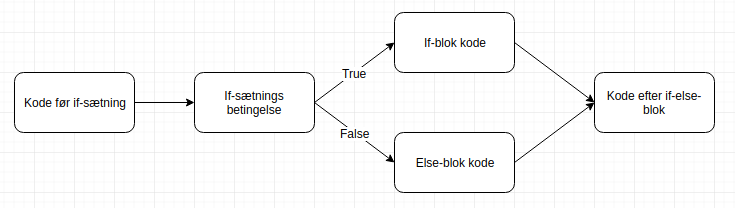
\includegraphics[width=0.9\textwidth]{if-else.png}
\end{center}

\end{frame}


\begin{frame}[fragile]{If-sætninger - at tage et valg}
Og med \texttt{elif} ser det således ud:
\begin{center}
	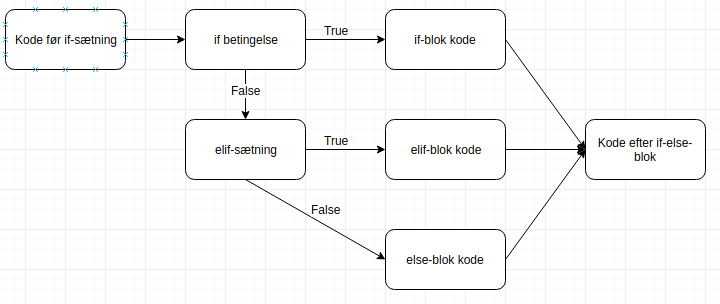
\includegraphics[width=0.9\textwidth]{if-elif-else.png}
\end{center}

Husk at der kan være lige så mange \texttt{elif}'s man har lyst, men den første der er sand vil blive valgt og de andre vil så ikke blive tjekket.

\end{frame}


\begin{frame}[fragile]{If-sætninger - at tage et valg}
	Måske skal der gælde mere end én ting før man vil gøre noget. F.eks. køber man kun bananen, hvis man både er over 18 og har penge nok. 
	\begin{lstlisting}[style=python]
age = 20
money = 42
	\end{lstlisting}
\end{frame}

\begin{frame}[fragile]{If-sætninger - at tage et valg}
	Måske skal der gælde mere end én ting før man vil gøre noget. F.eks. køber man kun bananen, hvis man både er over 18 og har penge nok. Her er en måde at løse det på:
	\begin{lstlisting}[style=python]
age = 20
money = 42
if (age >= 18):
	if (money >= 10):
		money = money - 10
		print("You bought an expensive banana")
	\end{lstlisting}
\end{frame}

\begin{frame}[fragile]{If-sætninger - at tage et valg}
	Der kan også være situationer, hvor bare én af flere ting er nok, for at udføre noget. F.eks. kan enten en fødselsdag eller en bommert være anledning til kage. Hvordan vil man så skrive sit program?
	\begin{lstlisting}[style=python]
birthday = False
blunder = True
	\end{lstlisting}
\end{frame}

\begin{frame}[fragile]{If-sætninger - at tage et valg}
	Der kan også være situationer, hvor bare én af flere ting er nok, for at udføre noget. F.eks. kan enten en fødselsdag eller en bommert være anledning til kage. Hvordan vil man så skrive sit program? Måske sådan her:
	\begin{lstlisting}[style=python]
birthday = False
blunder = True
caketime = False
if (birthday):
	caketime = True
if (blunder):
	caketime = True
	
if (caketime):
	print("It's cake time!")
	\end{lstlisting}
\end{frame}


\begin{frame}[fragile]{If-sætninger - at tage et valg}
	Heldigvis findes der en bedre måde. Man kan sammensætte boolske udtryk med \texttt{and} og \texttt{or}. Med \texttt{and} skal begge sider være opfyldt før det giver True, med \texttt{or} skal mindst én side være True før det giver True.
	\begin{lstlisting}[style=python]
age = 20
money = 42
if (age >= 18 and money >= 42):
	money = money - 10
	print("You bought an expensive banana")
	\end{lstlisting}
	
	\begin{lstlisting}[style=python]
birthday = False
blunder = True
if (birthday or blunder):
	print("It's cake time!")
	\end{lstlisting}
\end{frame}

%\begin{frame}[fragile]{If-sætninger - at tage et valg}
%	D
%\end{frame}




\section{Funktioner}

\begin{frame}[fragile]{Funktioner - undgå gentagelser}
	I har faktisk allerede brugt flere funktioner mange gange, f.eks. \texttt{print} og \texttt{type} funktionerne. At bruge en funktion hedder at man kalder funktionen, vi snakker altså om funktionskald. Man kan kende en funktion på at der er parenteser efter navnet.
	
	\begin{lstlisting}[style=python]
print("Hej")
type("Hej")
	\end{lstlisting}
	
	Det der står inde i parenteserne kaldes for parametre eller argumenter. Man kan også kalde det input til funktionen.
\end{frame}

\begin{frame}[fragile]{Funktioner - undgå gentagelser}
	Husk, man kan kombinere funktionskald. Så i stedet for:
	
	\begin{lstlisting}[style=python]
a = 3.14/2
a = int(a)
print(a)
	\end{lstlisting}
	
	Så kan man skrive:
	
	\begin{lstlisting}[style=python]
print(int(3.14/2))
	\end{lstlisting}
\end{frame}

\begin{frame}[fragile]{Funktioner - undgå gentagelser}
Forestil jer I har skrevet noget lækkert kode, men I skal hele tiden trække 1 fra og så printe værdien.
\begin{lstlisting}[style=python]
a = 7
b = a - 1
print(b)
c = (3**2 + 4**2)**0.5
d = c - 1
print(d)
e = 17 // 3
f = e - 1
print(f)
\end{lstlisting}
\end{frame}

\begin{frame}[fragile]{Funktioner - undgå gentagelser}
Forestil jer nu at I finder ud af at I skulle lægge 1 til i stedet for, så skal I finde alle de steder hvor I havde skrevet det og ændre det.
\begin{columns}
 	\column{0.4\textwidth}
	\begin{lstlisting}[style=python]
a = 7
b = a + 1
print(b)
c = (3**2 + 4**2)**0.5
d = c + 1
print(d)
e = 17 // 3
f = e + 1
print(f)
	\end{lstlisting}
	\column{0.4\textwidth}
	Output
	\begin{lstlisting}[style=python]
8
6.0
6
	\end{lstlisting}	
\end{columns}
\end{frame}


\begin{frame}[fragile]{Funktioner - undgå gentagelser}
Men programmører er dovne, vi kan gøre det smartere med funktioner:
\begin{columns}
	\column{0.4\textwidth}
	\begin{lstlisting}[style=python]
def newPrint(x):
	print(x+1)

a = 7
newPrint(a)
c = (3**2 + 4**2)**0.5
newPrint(c)
e = 17 // 3
newPrint(e)
	\end{lstlisting}
	\column{0.4\textwidth}
	Output
	\begin{lstlisting}[style=python]
8
6.0
6
	\end{lstlisting}	
\end{columns}
\end{frame}

\begin{frame}[fragile]{Funktioner - undgå gentagelser}
En funktion er opbygget således:
\begin{lstlisting}[style=python]
def <funktions navn>(<param. 1>, <param. 2>, ...):
	#kode
	return <værdi>
\end{lstlisting}
Hvis man har et \texttt{return} kan man sende et resultat tilbage og gemme/bruge til noget andet.
\end{frame}


\begin{frame}[fragile]{Funktioner - undgå gentagelser}
	Her er et eksempel på noget kode der udregner Pythagoras men som er copy-pastet rundt:
	\begin{lstlisting}[style=python]
a = 4
b = 2
c = (a**2 + b**2)**0.5
a = 3
b = 4
d = (a**2 + b**2)**0.5
	\end{lstlisting}
\end{frame}

\begin{frame}[fragile]{Funktioner - undgå gentagelser}
	Her er den samme kode, men hvor der er lavet en funktion istedet:
	\begin{lstlisting}[style=python]
def pyth(a, b):
	x = (a**2 + b**2)**0.5
	return x
c = pyth(4, 2)
d = pyth(3, 4)
	\end{lstlisting}

	Her var der to parametre i stedet for en, og vi gemte retur-værdien.
\end{frame}


\begin{frame}[fragile]{Funktioner - undgå gentagelser}
	En funktion behøver hverken have en retur værdi eller nogle parametre, den kan godt bare gøre det samme hver gang. F.eks.:
	\begin{lstlisting}[style=python]
def print_twice():
	s = "Hej med dig!"
	print(s)
	print(s)
	
print_twice()
	\end{lstlisting}
\end{frame}


\begin{frame}[fragile]{Recap}
	Hvad har vi set på i dette modul?
	\begin{itemize}
		\item Sammenligningsoperatorer
		\item if-else-sætninger
		\item 
	\end{itemize}
\end{frame}





% \begin{frame}{Metropolis titleformats}
%     \themename supports 4 different titleformats:
%     \begin{itemize}
%         \item Regular
%         \item \textsc{Smallcaps}
%         \item \textsc{allsmallcaps}
%         \item ALLCAPS
%     \end{itemize}
%     They can either be set at once for every title type or individually.
% \end{frame}

% {
%     \metroset{titleformat frame=smallcaps}
% \begin{frame}{Small caps}
%     This frame uses the \texttt{smallcaps} titleformat.

%     \begin{alertblock}{Potential Problems}
%         Be aware, that not every font supports small caps. If for example you typeset your presentation with pdfTeX and the Computer Modern Sans Serif font, every text in smallcaps will be typeset with the Computer Modern Serif font instead.
%     \end{alertblock}
% \end{frame}
% }

% {
% \metroset{titleformat frame=allsmallcaps}
% \begin{frame}{All small caps}
%     This frame uses the \texttt{allsmallcaps} titleformat.

%     \begin{alertblock}{Potential problems}
%         As this titleformat also uses smallcaps you face the same problems as with the \texttt{smallcaps} titleformat. Additionally this format can cause some other problems. Please refer to the documentation if you consider using it.

%         As a rule of thumb: Just use it for plaintext-only titles.
%     \end{alertblock}
% \end{frame}
% }

% {
% \metroset{titleformat frame=allcaps}
% \begin{frame}{All caps}
%     This frame uses the \texttt{allcaps} titleformat.

%     \begin{alertblock}{Potential Problems}
%         This titleformat is not as problematic as the \texttt{allsmallcaps} format, but basically suffers from the same deficiencies. So please have a look at the documentation if you want to use it.
%     \end{alertblock}
% \end{frame}
% }

% \section{Elements}

% \begin{frame}[fragile]{Typography}
%       \begin{verbatim}The theme provides sensible defaults to
% \emph{emphasize} text, \alert{accent} parts
% or show \textbf{bold} results.\end{verbatim}

%   \begin{center}becomes\end{center}

%   The theme provides sensible defaults to \emph{emphasize} text,
%   \alert{accent} parts or show \textbf{bold} results.
% \end{frame}

% \begin{frame}{Font feature test}
%   \begin{itemize}
%     \item Regular
%     \item \textit{Italic}
%     \item \textsc{SmallCaps}
%     \item \textbf{Bold}
%     \item \textbf{\textit{Bold Italic}}
%     \item \textbf{\textsc{Bold SmallCaps}}
%     \item \texttt{Monospace}
%     \item \texttt{\textit{Monospace Italic}}
%     \item \texttt{\textbf{Monospace Bold}}
%     \item \texttt{\textbf{\textit{Monospace Bold Italic}}}
%   \end{itemize}
% \end{frame}

% \begin{frame}{Lists}
%   \begin{columns}[T,onlytextwidth]
%     \column{0.33\textwidth}
%       Items
%       \begin{itemize}
%         \item Milk \item Eggs \item Potatos
%       \end{itemize}
%
%     \column{0.33\textwidth}
%       Enumerations
%       \begin{enumerate}
%         \item First, \item Second and \item Last.
%       \end{enumerate}
%
%     \column{0.33\textwidth}
%       Descriptions
%       \begin{description}
%         \item[PowerPoint] Meeh. \item[Beamer] Yeeeha.
%       \end{description}
%   \end{columns}
% \end{frame}
% \begin{frame}{Animation}
%   \begin{itemize}[<+- | alert@+>]
%     \item \alert<4>{This is\only<4>{ really} important}
%     \item Now this
%     \item And now this
%   \end{itemize}
% \end{frame}
% \begin{frame}{Figures}
%   \begin{figure}
%     \newcounter{density}
%     \setcounter{density}{20}
%     \begin{tikzpicture}
%       \def\couleur{alerted text.fg}
%       \path[coordinate] (0,0)  coordinate(A)
%                   ++( 90:5cm) coordinate(B)
%                   ++(0:5cm) coordinate(C)
%                   ++(-90:5cm) coordinate(D);
%       \draw[fill=\couleur!\thedensity] (A) -- (B) -- (C) --(D) -- cycle;
%       \foreach \x in {1,...,40}{%
%           \pgfmathsetcounter{density}{\thedensity+20}
%           \setcounter{density}{\thedensity}
%           \path[coordinate] coordinate(X) at (A){};
%           \path[coordinate] (A) -- (B) coordinate[pos=.10](A)
%                               -- (C) coordinate[pos=.10](B)
%                               -- (D) coordinate[pos=.10](C)
%                               -- (X) coordinate[pos=.10](D);
%           \draw[fill=\couleur!\thedensity] (A)--(B)--(C)-- (D) -- cycle;
%       }
%     \end{tikzpicture}
%     \caption{Rotated square from
%     \href{http://www.texample.net/tikz/examples/rotated-polygons/}{texample.net}.}
%   \end{figure}
% \end{frame}
% \begin{frame}{Tables}
%   \begin{table}
%     \caption{Largest cities in the world (source: Wikipedia)}
%     \begin{tabular}{lr}
%       \toprule
%       City & Population\\
%       \midrule
%       Mexico City & 20,116,842\\
%       Shanghai & 19,210,000\\
%       Peking & 15,796,450\\
%       Istanbul & 14,160,467\\
%       \bottomrule
%     \end{tabular}
%   \end{table}
% \end{frame}
% \begin{frame}{Blocks}
%   Three different block environments are pre-defined and may be styled with an
%   optional background color.

%   \begin{columns}[T,onlytextwidth]
%     \column{0.4\textwidth}
%       \begin{block}{Default}
%         Block content.
%       \end{block}

%       \begin{alertblock}{Alert}
%         Block content.
%       \end{alertblock}

%       \begin{exampleblock}{Example}
%         Block content.
%       \end{exampleblock}

%     \column{0.4\textwidth}

%       \metroset{block=fill}

%       \begin{block}{Default}
%         Block content.
%       \end{block}

%       \begin{alertblock}{Alert}
%         Block content.
%       \end{alertblock}

%       \begin{exampleblock}{Example}
%         Block content.
%       \end{exampleblock}

%   \end{columns}
% \end{frame}
% \begin{frame}{Math}
%   \begin{equation*}
%     e = \lim_{n\to \infty} \left(1 + \frac{1}{n}\right)^n
%   \end{equation*}
% \end{frame}
% \begin{frame}{Line plots}
%   \begin{figure}
%     \begin{tikzpicture}
%       \begin{axis}[
%         mlineplot,
%         width=0.9\textwidth,
%         height=6cm,
%       ]

%         \addplot {sin(deg(x))};
%         \addplot+[samples=100] {sin(deg(2*x))};

%       \end{axis}
%     \end{tikzpicture}
%   \end{figure}
% \end{frame}
% \begin{frame}{Bar charts}
%   \begin{figure}
%     \begin{tikzpicture}
%       \begin{axis}[
%         mbarplot,
%         xlabel={Foo},
%         ylabel={Bar},
%         width=0.9\textwidth,
%         height=6cm,
%       ]

%       \addplot plot coordinates {(1, 20) (2, 25) (3, 22.4) (4, 12.4)};
%       \addplot plot coordinates {(1, 18) (2, 24) (3, 23.5) (4, 13.2)};
%       \addplot plot coordinates {(1, 10) (2, 19) (3, 25) (4, 15.2)};

%       \legend{lorem, ipsum, dolor}

%       \end{axis}
%     \end{tikzpicture}
%   \end{figure}
% \end{frame}
% \begin{frame}{Quotes}
%   \begin{quote}
%     Veni, Vidi, Vici
%   \end{quote}
% \end{frame}

% {%
% \setbeamertemplate{frame footer}{My custom footer}
% \begin{frame}[fragile]{Frame footer}
%     \themename defines a custom beamer template to add a text to the footer. It can be set via
%     \begin{verbatim}\setbeamertemplate{frame footer}{My custom footer}\end{verbatim}
% \end{frame}
% }

% \begin{frame}{References}
%   Some references to showcase [allowframebreaks] \cite{knuth92,ConcreteMath,Simpson,Er01,greenwade93}
% \end{frame}

% \section{Conclusion}

% \begin{frame}{Summary}

%   Get the source of this theme and the demo presentation from

%   \begin{center}\url{github.com/matze/mtheme}\end{center}

%   The theme \emph{itself} is licensed under a
%   \href{http://creativecommons.org/licenses/by-sa/4.0/}{Creative Commons
%   Attribution-ShareAlike 4.0 International License}.

%   \begin{center}\ccbysa\end{center}

% \end{frame}

% {\setbeamercolor{palette primary}{fg=black, bg=Orange}
% \begin{frame}[standout]
%   Questions?
% \end{frame}
% }

% \appendix

% \begin{frame}[fragile]{Backup slides}
%   Sometimes, it is useful to add slides at the end of your presentation to
%   refer to during audience questions.

%   The best way to do this is to include the \verb|appendixnumberbeamer|
%   package in your preamble and call \verb|\appendix| before your backup slides.

%   \themename will automatically turn off slide numbering and progress bars for
%   slides in the appendix.
% \end{frame}

% \begin{frame}[allowframebreaks]{References}

%   \bibliography{demo}
%   \bibliographystyle{abbrv}

% \end{frame}

\end{document}